\subsection{Иерархия удостоверяющих центров}\label{section-CAs}
\selectlanguage{russian}

Проблему аутентификации и распределения сеансовых симметричных ключей шифрования в Интернете, а также в больших локальных и виртуальных сетях, решают с помощью построения иерархии открытых ключей криптосистем с открытым ключом.

\begin{enumerate}
    \item Существует удостоверяющий центр (УЦ) верхнего уровня\index{Удостоверяющий центр!верхнего уровня}, корневой УЦ\index{Удостоверяющий центр!корневой} (Root Certification Authority, $CA$)\index{Certification Authority!Root}, обладающий парой из секретного и открытого ключей. Открытый ключ УЦ верхнего уровня распространяется среди всех пользователей, причем все пользователи \emph{доверяют УЦ}. Это означает, что:
        \begin{itemize}
            \item УЦ -- <<хороший>>, обеспечивает надежное хранение секретного ключа, не пытается фальсифицировать и скомпрометировать свои ключи,
            \item имеющийся у пользователей открытый ключ УЦ действительно принадлежит УЦ.
        \end{itemize}
        В массовых информационных и интернет-системах открытые ключи многих корневых УЦ встроены в дистрибутивы и пакеты обновлений ПО. Доверие пользователей неявно проявляется в их уверенности в том, что открытые ключи корневых УЦ, включенные в ПО, не фальсифицированы и не скомпрометированы. \emph{Де-факто пользователи доверяют а) распространителям ПО и обновлений, б) корневому УЦ.}\index{доверие}

        Назначение УЦ верхнего уровня -- проверка принадлежности и подписание открытых ключей других удостоверяющих центров второго уровня, а также организаций и сервисов. УЦ подписывает своим секретным ключом следующее сообщение:
        \begin{itemize}
            \item название и URI УЦ нижележащего уровня или организации/сервиса,
            \item значение сгенерированного открытого ключа и название алгоритма соответствующей криптосистемы с открытым ключом,
            \item время выдачи и срок действия открытого ключа.
        \end{itemize}

    \item УЦ второго уровня (certificate authority, CA) имеют свои пары открытых и секретных ключей, сгенерированных и подписанных корневым УЦ. Причем перед подписанием корневой УЦ убеждается в <<надежности>> УЦ второго уровня, производит юридические проверки. Корневой УЦ не имеет доступа к секретным ключам УЦ второго уровня.

        Пользователи, имея в своей базе открытых ключей доверенные открытые ключи корневого УЦ, могут проверить ЭП открытых ключей УЦ 2-го уровня и убедиться, что предъявленный открытый ключ действительно принадлежит данному УЦ. Таким образом:
        \begin{itemize}
            \item Пользователи полностью доверяют корневому УЦ и его открытому ключу, который у них хранится. Пользователи верят, что корневой УЦ не подписывает небезопасные ключи и гарантирует, что подписанные им ключи действительно принадлежат УЦ 2-го уровня.
            \item Проверив ЭП открытого ключа УЦ 2-го уровня с помощью доверенного открытого ключа УЦ 1-го уровня, пользователь верит, что открытый ключ УЦ 2-го уровня действительно принадлежит данному УЦ и не был скомпрометирован.
        \end{itemize}

        Аутентификация в протоколе защищенного интернет-соединения SSL/TLS\index{протокол!SSL/TLS} достигается в результате проверки пользователями совпадения URI-адреса сервера из ЭП с фактическим адресом.

        УЦ второго уровня в свою очередь тоже подписывает открытые ключи УЦ третьего уровня, а также организаций. И так далее по уровням.

    \item В результате построена \emph{иерархия} подписанных открытых ключей.

    \item Открытый ключ с идентификационной информацией (название организации, URI-адрес вебресурса, дата выдачи, срок действия и др.) и подписью УЦ вышележащего уровня, заверяющей ключ и идентифицирующие реквизиты, называется \textbf{сертификатом открытого ключа},\index{сертификат открытого ключа} на который существует международный стандарт X.509, последняя версия 3. В сертификате указывается его область применения: подписание других сертификатов, аутентификация для веба, аутентификация для электронной почты и т.д.
\end{enumerate}


\begin{figure}[!ht]
	\centering
	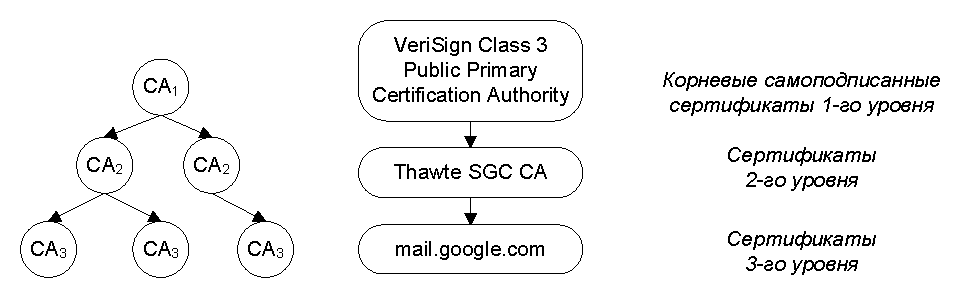
\includegraphics[width=0.8\textwidth]{pic/X509-hierarchy}
	\caption{Иерархия сертификатов\label{fig:x509-hierarchy}}
\end{figure}

На рис. \ref{fig:x509-hierarchy} приведены пример иерархии сертификатов и путь подписания сертификата X.509 интернет-сервиса Google Mail.

Система распределения, хранения и управления сертификатами открытых ключей называется \textbf{инфраструктурой открытых ключей}\index{инфраструктура открытых ключей} (public key infrastructure, PKI)\index{PKI}. PKI применяется для аутентификации в системах SSL/TLS\index{протокол!SSL/TLS}, IPsec\index{протокол!IPsec}, PGP\index{PGP} и т.д. Помимо процедур выдачи и распределения открытых ключей PKI также определяет процедуру отзыва скомпрометированных или устаревших сертификатов.
